\section{Results}\label{sec:results}

We proceed from validating the triage, to the headline remedy decomposition (the
deficit is mostly threshold-recoverable), to the mechanism (controlled overlap and
a proposition), to its consequence at scale (oversampling is an operating-point
move: no ranking gain, worse calibration, and a tie with threshold-moving at
parity), and finally to the prescription (a regime map and an honestly-scoped
selector).

\subsection{Error Instance Triage: validation}\label{sec:results:validation}

\paragraph{Synthetic ground truth.} On two-class Gaussian mixtures the triage
behaves as designed. As class separation shrinks from $1.2$ to $0.2$ standard
deviations (overlap grows), the Cat\,3 (irreducible) fraction among errors rises
monotonically, exceeding $95\%$ at the smallest separation (mean $94.3\%$ across
the sweep) --- the triage correctly attributes boundary-overlap errors to
irreducibility. On 24 real datasets with $5\%$ injected label noise the triage
detects the flips with mean precision $0.77$, and the flagged-noise fraction rises
significantly ($p=2\times10^{-5}$, Wilcoxon). The triage is thus sensitive to both
boundary overlap (Cat\,3) and label noise (Cat\,1), the two categories that drive
the mechanism below.

\paragraph{Out-of-fold robustness.} Because the categories underpin the mechanistic
argument, we verify they are not in-sample artefacts. The category assignment
already uses out-of-bag predictions (\S\ref{sec:method:uncert}); under a strict
inner cross-validation that re-derives \emph{every} signal --- including the
aleatoric/epistemic decomposition --- on held-out instances, the Cat\,3 fraction
among errors is essentially unchanged (in-sample $\to$ out-of-fold mean shift of
$\approx\!\OOFCATSHIFT$\,pp over 79 datasets) and the aleatoric/epistemic ordering
that defines the categories is preserved (\appref{app:oof}).

\paragraph{Is the triage a uniquely good predictor of SMOTE harm? No --- and it
need not be.} A reviewer will rightly ask whether the aleatoric--epistemic triage
is necessary or whether a simpler $k$-NN hardness / overlap score localizes
SMOTE's harm equally well. Across the 75 datasets with a SMOTE outcome we correlate
eleven per-dataset measures with SMOTE's accuracy cost (Table~\ref{tab:ablation}).
The trivial \emph{minority error rate} is the strongest single predictor
($\rho=-0.49$, leave-one-out $R^2=0.34$), with the Napiera{\l}a rare/outlier
fraction and the imbalance ratio close behind ($\rho\approx-0.40$); the triage's
Cat\,3 mass is only a moderate, marginally significant predictor ($\rho=-0.21$,
$p=0.07$). The \emph{conditional} Cat\,3 fraction (\texttt{frac\_cat3}) even
correlates with \emph{less} accuracy harm ($\rho=+0.37$): the fraction of errors
that are boundary errors is not the dataset-level \emph{mass} of boundary-entangled
minority, and a dataset can carry a high Cat\,3 share within a \emph{small} error
population --- a near-ceiling problem SMOTE barely perturbs. The mechanism is tied
to that boundary mass (better captured by the minority error rate), not the
conditional fraction alone. We state this plainly: the triage is \emph{not} a better
cross-dataset forecaster of SMOTE harm than simple measures, and we do not claim it
is. Its role
is \emph{explanatory} --- it localizes \emph{which} errors lie in the
boundary/overlap region so the intervention of
\S\ref{sec:results:interventional} can seed augmentation there and probe the
mechanism --- not a predictive instrument, consistent with the honest selection
finding of \S\ref{sec:results:selection}. Put differently, the minority error rate
predicts the \emph{size} of the deficit; the remedy decomposition diagnoses the
\emph{appropriate intervention}.

\begin{table}[t]
\centering
\caption{Triage-design ablation: Spearman correlation of each per-dataset measure
with SMOTE's accuracy change ($\Delta$acc) and balanced-accuracy change
($\Delta$bacc), and a single-feature leave-one-out $R^2$ for $\Delta$acc, over 75
datasets. The triage's Cat\,3 mass is not a stronger predictor of SMOTE harm than
simple hardness/imbalance measures; the triage's value is explanatory, not
predictive. $^{*}$: $p<0.05$.}
\label{tab:ablation}
\begin{tabular}{lrrr}
\toprule
Per-dataset measure & $\rho$(SMOTE $\Delta$acc) & $\rho$($\Delta$bacc) & LOO $R^2$($\Delta$acc) \\
\midrule
minority error rate & -0.49$^{*}$ & +0.57 & 0.34 \\
Napierala rare+outlier & -0.40$^{*}$ & +0.58 & 0.17 \\
imbalance ratio & -0.40$^{*}$ & +0.76 & -0.23 \\
frac\_cat3 (triage) & +0.37$^{*}$ & -0.53 & -0.00 \\
LOO 1-NN error (N3) & -0.24$^{*}$ & -0.06 & -0.01 \\
cat3\_mass (triage) & -0.21 & -0.12 & -0.01 \\
boundary frac (N1) & -0.20 & -0.15 & -0.02 \\
Fisher F1 & -0.13 & +0.45 & 0.01 \\
instance hardness (max\_fdr) & +0.13 & -0.45 & -0.04 \\
intra/extra ratio (N2) & +0.06 & +0.34 & -0.03 \\
Napierala borderline & +0.02 & +0.04 & -0.03 \\
\bottomrule
\end{tabular}

\end{table}

\subsection{The minority deficit is mostly threshold-recoverable}\label{sec:results:remedy}

\paragraph{Result.} We apply the remedy decomposition (\S\ref{sec:method:remedy})
to the misclassified minority on every dataset (Table~\ref{tab:reducibility}).
Across the 70 datasets with a non-trivial minority error set, the deficit is
\textbf{predominantly threshold-recoverable}: a mean of $\mathbf{69\%}$ (median
$75\%$) of minority errors are corrected simply by moving the decision threshold to
its out-of-fold balanced-accuracy optimum --- the model already \emph{ranked} these
instances correctly. Only $7\%$ are data-reducible (epistemic --- where more
same-class data would help), $16\%$ are irreducible (aleatoric --- model-estimated
overlap), and $7\%$ are noise. The pattern \emph{sharpens} with imbalance: on
$\mathrm{IR}>3$ datasets $74\%$ of the deficit is threshold-recoverable. This is
corroborated independently by separability: on the 30 hardest binary datasets
(baseline balanced accuracy $<0.85$) the baseline classifier's out-of-fold AUC is a
median of $0.91$ ($93\%$ exceed $0.70$) --- the classes are well ranked even where
default-threshold balanced accuracy is poor. (The genuine exceptions, AUC
$\approx0.59$, are the near-irreducible problems.)

\paragraph{Consistency with Cat\,3 dominating the errors.} The $\sim$85\% Cat\,3
share reported below (\S\ref{sec:results:interventional}) and the $16\%$ irreducible
fraction here are not in tension (\S\ref{sec:method:remedy}). Cat\,3 is a triage
label for errors in the estimated overlap region under the \emph{default} decision
rule, computed over \emph{all} errors; the remedy decomposition then asks, for the
\emph{minority} errors only, whether that default-threshold mistake survives a move
to the tuned operating point $\tau^\star$. Because the classifier ranks most of
these boundary errors above $\tau^\star$, they are counted threshold-recoverable,
and only the residue the threshold move cannot rescue is counted irreducible --- a
strict subset of the minority Cat\,3 errors, not the whole category.

\begin{table}[t]
\centering
\caption{Remedy decomposition of the misclassified minority (mean over datasets,
out-of-bag): the fraction of minority errors that are threshold-recoverable (a
threshold move corrects them), data-reducible (epistemic; more minority data
helps), irreducible (aleatoric; model-estimated overlap), or noise. The deficit is
predominantly a thresholding artefact, increasingly so with imbalance.}
\label{tab:reducibility}
\begin{tabular}{lrrrr}
\toprule
Subset & threshold-recoverable & data-reducible & irreducible & noise \\
\midrule
All datasets & 68\% & 6\% & 17\% & 9\% \\
$\mathrm{IR}>3$ & 80\% & 4\% & 5\% & 12\% \\
$\mathrm{IR}>10$ & 80\% & 5\% & 2\% & 13\% \\
Binary & 69\% & 4\% & 15\% & 12\% \\
Multiclass & 67\% & 10\% & 22\% & 1\% \\
\bottomrule
\end{tabular}

\end{table}

\paragraph{Why this matters.} This decomposition is the mechanistic account of a
well-documented but unexplained regularity --- that resampling does not improve
ranking and a threshold move reproduces its benefit
\cite{provost2000imbalanced,elkan2001foundations,elor2022smote,goorbergh2022harm}.
\emph{Because} most of the minority deficit is threshold-recoverable, a
non-generative change of the decision rule recovers it, and oversampling --- which
leaves ranking unchanged (\S\ref{sec:results:frontier}) --- is at best an implicit,
inefficient way to enact the same threshold move. The decomposition also tells a
practitioner \emph{which} situation they are in: the (minority) data-reducible
fraction is where collecting or generating minority data is warranted; the
irreducible fraction is where no remedy in our evaluated menu helps.

\subsection{Mechanism: SMOTE generates across the Bayes boundary}\label{sec:results:mechanism}

\paragraph{Premise.} If SMOTE's accuracy cost arises from generation near the
Bayes boundary, then on a controlled problem with a \emph{known} boundary,
standard SMOTE should place synthetic minority points \emph{across} that boundary
--- in majority territory, where they act as label noise --- increasingly so as
overlap grows, while excluding the irreducible seeds should prevent it.

\paragraph{Result.} We generate 2D Gaussian classes
($\mathcal{N}([\pm s,0], I)$, $9{:}1$ imbalance, balanced Bayes boundary
$x=0$) and sweep the separation $s$. Standard SMOTE places an
\emph{overlap-dependent} fraction of its synthetic minority points on the
majority side of the boundary --- from $6\%$ at $s=1.5$ to $34\%$ at $s=0.4$ ---
whereas masking the Cat\,3 (boundary) seeds generates essentially none
($\le 2\%$, $0\%$ for $s\ge0.8$); Figure~\ref{fig:overlap} visualizes both.

\begin{figure}[t]
\centering
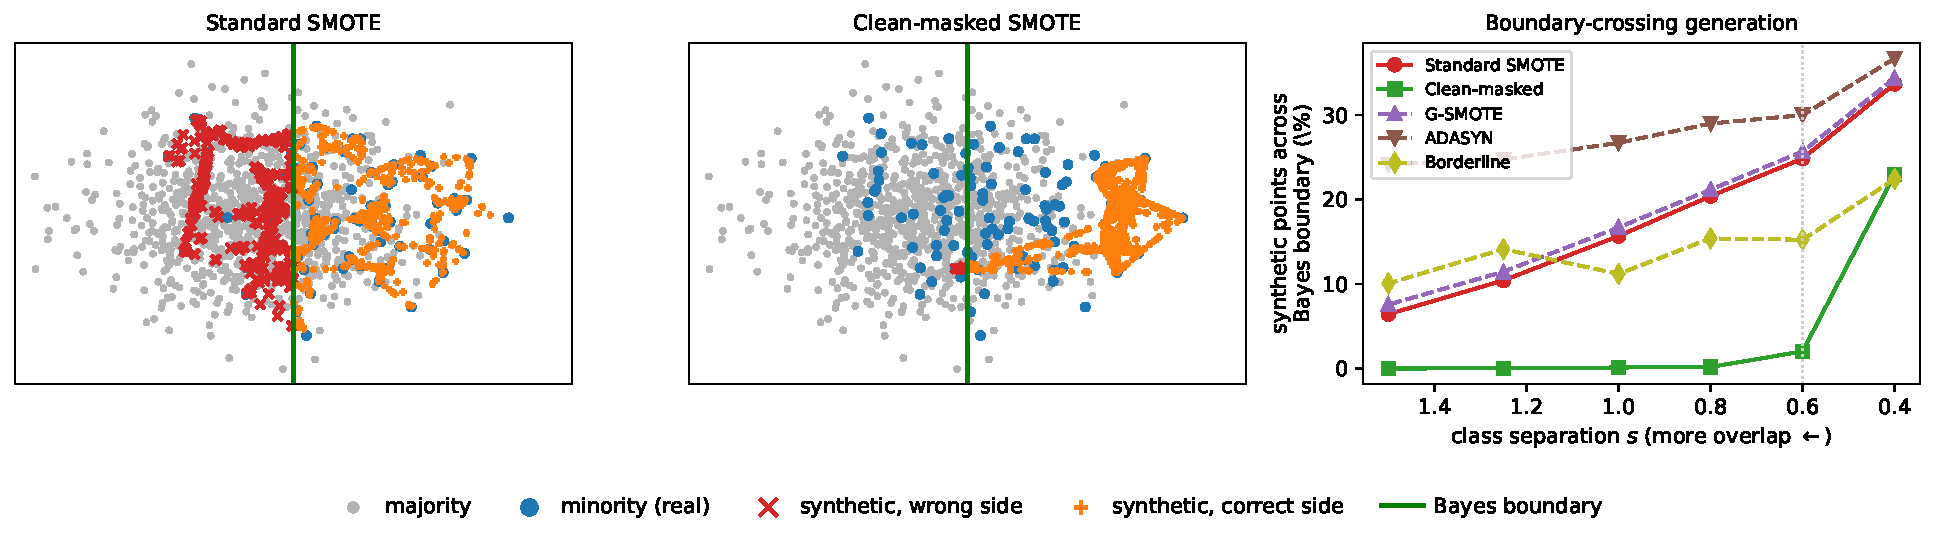
\includegraphics[width=\linewidth]{figures/fig_overlap.pdf}
\caption{Mechanism on controlled 2D Gaussians ($9{:}1$; balanced Bayes boundary
$x=0$, green). Left/middle: at moderate overlap ($s=0.6$) standard SMOTE scatters
synthetic minority points (red $\times$) across the boundary into majority
territory; masking the boundary seeds keeps generation on the minority side.
Right: the fraction of synthetic points crossing the boundary rises with overlap
for SMOTE but stays near zero when boundary seeds are excluded.}
\label{fig:overlap}
\end{figure}

\subsection{Interventional evidence}\label{sec:results:interventional}

\paragraph{Premise.} If the accuracy--balanced-accuracy tradeoff is \emph{caused}
by generation near the (estimated) boundary, then targeted generation around
Cat\,3 (irreducible) errors should reproduce the SMOTE signature, while
random-instance generation should not.

\paragraph{Protocol.} On each training fold we compute the triage and, for each
strategy, append a \emph{fixed} budget $B$ of synthetic points equal to the total
number of triage errors on that fold --- identical across strategies, so the
comparison isolates \emph{where} one generates, not how much. Synthetic points are
produced by SMOTE-style interpolation \emph{within the targeted seed subset only}
(each synthetic point takes its seed's own class, with $B$ split across classes in
proportion to the seed subset's class distribution); all original training instances
are kept, and the data are \emph{not} rebalanced to a fixed ratio. The six
strategies are: \texttt{augment\_cat2} and \texttt{augment\_cat3} (seeds from the
respective error category), \texttt{augment\_all\_errors} (all errors),
\texttt{augment\_random} (a size-$B$ random sample of \emph{all} training instances
--- class-proportional, hence a true null that cannot shift the class balance), and
two removal controls (\texttt{remove\_noise}, \texttt{remove\_random}). The base
learner is XGBoost; metrics are over $5\times5$ folds. Seeds come from the triage on
the training fold. This real-data intervention is a \emph{small} effect and, as we
report honestly, sensitive to seed re-estimation (\appref{app:oof}); we treat
it as corroboration of, not primary evidence for, the mechanism --- which rests on
the controlled experiment (\S\ref{sec:results:mechanism}, known boundary) and the
discrimination/threshold analysis (\S\ref{sec:results:frontier}).

\paragraph{Result.} We run these strategies on each of 50 datasets against a
no-augmentation baseline. Augmenting Cat\,3 errors
recreates the signature tradeoff: balanced accuracy improves (win rate $68\%$,
$p=0.001$) while accuracy trends negative. Augmenting all errors amplifies it
($p<0.001$) because Cat\,3 dominates the error population ($\sim$86\%). Crucially,
\emph{random} augmentation produces no effect on either metric (WR $\approx50\%$,
$p>0.5$), and augmenting Cat\,2 errors helps balanced accuracy modestly
($p=0.007$) without harming accuracy (Figure~\ref{fig:interventional}).

\begin{figure}[t]
\centering
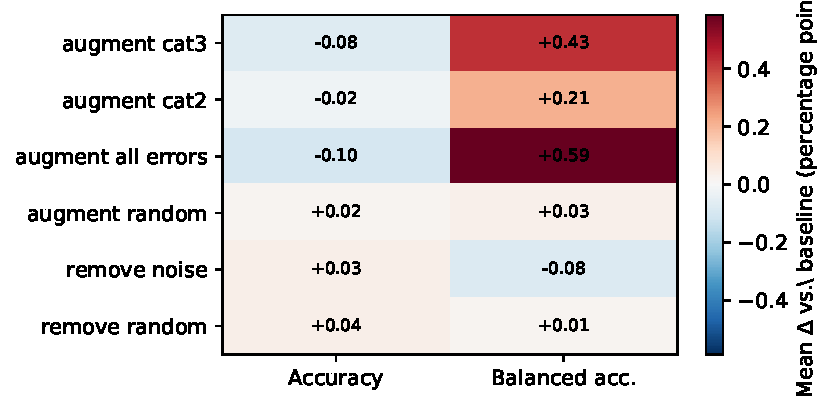
\includegraphics[width=\linewidth]{figures/fig1_interventional.pdf}
\caption{Interventional validation: mean metric change vs.\ the no-augmentation
baseline by augmentation target (50 datasets, fixed budget). Cat\,3
(boundary) augmentation reproduces the SMOTE signature --- balanced-accuracy gain
at an accuracy cost --- while random augmentation is null.}
\label{fig:interventional}
\end{figure}

\paragraph{Interpretation.} Consistent with the mechanism, the targeted-augmentation
contrast points to generation in the model-estimated boundary/overlap region
(Cat\,3) as the source of the accuracy cost, with the random-augmentation control
null. We are deliberately measured here: this is a \emph{small} real-data effect
that manipulates \emph{model-estimated} hard instances (not the true, unobserved
Bayes boundary), and it weakens under strict out-of-fold seed re-estimation at
reduced power (\appref{app:oof}). The mechanism does not rest on it: the
controlled experiment of \S\ref{sec:results:mechanism} (known boundary) and the
discrimination/threshold analysis of \S\ref{sec:results:frontier} (oversampling
does not improve ranking; its gain is a recoverable operating-point shift) are the
load-bearing evidence.

\subsection{Oversampling is an operating-point move, not a discrimination gain}\label{sec:results:frontier}

We now confirm the consequence the decomposition predicts, on the full menu and at
scale. The results in this section reproduce known findings
\cite{provost2000imbalanced,elor2022smote,goorbergh2022harm,dalpozzolo2015calibrating}
on a broad roster; we present them as confirmation that grounds the mechanism, not
as new claims.

\paragraph{No discrimination gain; worse calibration.} Oversampling does not help
the classifier \emph{rank}: on the binary datasets, SMOTE's out-of-fold ROC-AUC
($0.911$) and PR-AUC (at fixed test prevalence, $0.653$) are statistically
indistinguishable from the unresampled baseline ($0.909$, $0.655$), while its
probability calibration is worse (Brier $0.031$ vs.\ $0.028$; expected calibration
error $0.030$ vs.\ $0.025$), with Safe-Level-SMOTE worst (Table~\ref{tab:metrics}).
This matches the established account that resampling leaves ranking intact and
shifts only the threshold-dependent operating point, at a calibration cost
\cite{dalpozzolo2015calibrating,goorbergh2022harm,carriero2025harms}. Whatever
balanced-accuracy SMOTE buys is therefore an operating-point move, not a better
classifier.

\paragraph{At threshold parity, oversampling adds little.} The headline ``win''
of non-generative strategies is itself an operating-point artefact. At the
\emph{default} threshold, non-generative strategies top the balanced-accuracy
ranking on both rosters (best non-gen $\ge$ best gen on balanced accuracy in
$25/27$ KEEL datasets, $+5.76$\,pp, $95\%$ CI $[+3.81,+7.90]$; $43/52$ OpenML,
$+2.02$\,pp, $[+1.20,+2.98]$; $86\%$ overall; Friedman--Nemenyi
Figure~\ref{fig:cd}, $\chi^2{=}285.6$, $p<10^{-50}$, threshold-moving best rank
$3.15$) --- but only because threshold-moving is tuned and the SMOTE family is
scored at $0.5$. When \emph{every} strategy receives the same out-of-fold
threshold tuning, almost the entire gap disappears: on the 27 KEEL binary datasets
a tuned threshold alone lifts SMOTE's balanced accuracy by $+6.4$\,pp, and the
best-non-generative\,$-$\,best-generative difference collapses from $+5.76$\,pp at
the default threshold to within $\pm1$\,pp at parity (Table~\ref{tab:parity}:
$-0.72$\,pp for XGBoost, $-0.49$ for RF, $+0.19$ for logistic regression). We are
precise about the residual: at parity the best \emph{generative} strategy is in
fact marginally \emph{ahead} on XGBoost ($0.72$\,pp, $p{=}0.003$) and RF
($p{=}0.06$), and tied on logistic regression --- but this sub-$1$\,pp edge comes
with \emph{no} ranking gain and \emph{worse} calibration (above), against a
$+6.4$\,pp threshold effect. The decisive lever is therefore the \emph{threshold},
not the generative/non-generative choice, which is a fraction of its size. This
corroborates, on a 16-strategy menu and three learners, the broader-roster
conclusion of \cite{elor2022smote} (73 datasets) and \cite{goorbergh2022harm} that
balancing and threshold-tuning yield equivalent discrimination.

\begin{table}[t]
\centering
\caption{Probability metrics by strategy (XGBoost, mean over the 27 KEEL binary
datasets, out-of-fold). Oversampling does not improve ranking (ROC-AUC, PR-AUC at
fixed prevalence) and worsens calibration (Brier, expected calibration error);
recall at $10\%$ false-positive rate is likewise unimproved.}
\label{tab:metrics}
\small
\begin{tabular}{lrrrrrrr}
\toprule
 & none & cost & SMOTE & Border & ADASYN & SafeLvl & G-SMOTE \\
\midrule
ROC-AUC & 0.909 & 0.905 & 0.911 & 0.910 & 0.910 & 0.905 & 0.908 \\
PR-AUC & 0.655 & 0.652 & 0.653 & 0.650 & 0.649 & 0.632 & 0.649 \\
Brier & 0.028 & 0.034 & 0.031 & 0.031 & 0.032 & 0.040 & 0.031 \\
Brier (bal.) & 0.205 & 0.169 & 0.169 & 0.175 & 0.168 & 0.160 & 0.186 \\
ECE & 0.025 & 0.035 & 0.030 & 0.029 & 0.031 & 0.044 & 0.030 \\
ECE (bal.) & 0.233 & 0.182 & 0.185 & 0.192 & 0.185 & 0.170 & 0.209 \\
Rec@FPR10 & 0.775 & 0.766 & 0.774 & 0.775 & 0.773 & 0.751 & 0.773 \\
ROC-AUC rank & 4.02 & 4.94 & 3.65 & 3.76 & 3.65 & 4.74 & 3.24 \\
Brier rank & 2.63 & 3.93 & 3.85 & 4.04 & 4.59 & 6.00 & 2.96 \\
\bottomrule
\end{tabular}

\end{table}

\begin{table}[t]
\centering
\caption{Threshold parity: best non-generative $-$ best generative balanced
accuracy when \emph{every} strategy is given the same out-of-fold threshold tuning,
per base learner (27 KEEL binary datasets). The difference is within $\pm1$\,pp on
every learner (a small generative edge on XGBoost/RF, tied on logistic regression),
versus a $+5.76$\,pp non-generative advantage at the default threshold --- the
default-threshold ``dominance'' is overwhelmingly an operating-point effect.}
\label{tab:parity}
\begin{tabular}{lrrrr}
\toprule
Base learner & $n$ & NG$\ge$G & non-gen advantage & paired $p$ \\
\midrule
XGBoost & 27 & 19\% & $-0.72$ [-1.52,-0.18] & $0.003$ \\
Random forest & 26 & 27\% & $-0.49$ [-1.11,-0.03] & $0.06$ \\
Logistic regression & 27 & 59\% & $+0.19$ [-0.06,+0.43] & $0.2$ \\
\bottomrule
\end{tabular}

\end{table}

\paragraph{The default-threshold gap scales with imbalance.} Because the deficit
grows with imbalance, so does the (operating-point) penalty of leaving SMOTE at the
default threshold (Table~\ref{tab:irstrata}): the default-threshold non-generative
advantage rises from $+4.45$\,pp at $\mathrm{IR}>1.5$ to $+5.78$\,pp at
$\mathrm{IR}>10$, and SMOTE's accuracy cost deepens in lockstep ($-0.37 \to
-0.72$\,pp) as its balanced-accuracy gain grows ($+2.30 \to +4.28$\,pp). The
tradeoff is dose-responsive to imbalance, exactly as the boundary mechanism
predicts; the parity result above shows this default-threshold gap is recoverable
by a threshold move rather than by generation.

\paragraph{The cost tracks the mechanism.} SMOTE's per-dataset accuracy loss scales
with the minority error rate ($\rho=-0.50$, $p<10^{-4}$) and the imbalance ratio
($\rho=-0.41$, $p<10^{-3}$): it hurts most exactly where the minority is most
boundary-entangled and rebalancing is most aggressive --- the regime the mechanism
predicts.

\begin{table}[t]
\centering
\caption{The default-threshold non-generative advantage and the SMOTE tradeoff by
data stratum (existing benchmark cells, no re-run), all at the \emph{default}
threshold. NG$\ge$G is the fraction of datasets where the best non-generative
strategy matches/beats the best generative one on balanced accuracy; ``bacc adv.''
is the mean per-dataset advantage; the last two columns are SMOTE's mean accuracy
and balanced-accuracy change vs.\ the do-nothing baseline (percentage points). The
gap grows with imbalance but is an operating-point effect (Table~\ref{tab:parity}).}
\label{tab:irstrata}
\begin{tabular}{lrrrrr}
\toprule
Subset & $n$ & NG$\ge$G & bacc adv. & SMOTE $\Delta$acc & SMOTE $\Delta$bacc \\
\midrule
$\mathrm{IR}>1.5$ & 53 & 87\% & +4.45 & -0.56 & +3.20 \\
$\mathrm{IR}>3$ & 44 & 89\% & +5.27 & -0.61 & +3.72 \\
$\mathrm{IR}>10$ & 32 & 88\% & +5.78 & -0.72 & +4.28 \\
binary only & 46 & 85\% & +4.35 & -0.35 & +2.96 \\
multiclass only & 29 & 90\% & +1.86 & -0.39 & +1.24 \\
high-overlap & 26 & 77\% & +1.68 & -0.42 & +1.45 \\
\bottomrule
\end{tabular}

\end{table}

\paragraph{Not a base-learner artefact.} The pattern is not specific to
gradient-boosted trees. With random-forest and logistic-regression base learners
the default-threshold non-generative advantage persists ($+2.07$\,pp, $75\%$,
$p=1.6\times10^{-4}$ for RF; $+6.44$\,pp, $96\%$, $p=2\times10^{-10}$ for logistic
regression, the most miscalibrated learner) --- and the threshold-parity analysis
(Table~\ref{tab:parity}) likewise holds across all three learners, confirming the
gap is an operating-point effect rather than a property of any one model family.

\begin{table}[!tp]
\centering
\caption{Per-strategy mean accuracy / balanced accuracy across the 16-strategy
menu (XGBoost base learner; KEEL, $n{=}27$; OpenML, $n{=}52$), sorted by mean
balanced accuracy. \emph{At the default decision threshold}, non-generative
strategies ($\dagger$) occupy the top of the balanced-accuracy ranking on both
rosters and the entire SMOTE family sits below them, but this ranking gap is
largely an operating-point effect that collapses once every strategy receives the
same out-of-fold threshold tuning (Table~\ref{tab:parity}). Entries are means
over the $25$ folds; ``rank'' is the mean
per-dataset balanced-accuracy rank over the full menu on the $N{=}46$ binary
datasets (lower is better; the ranking of Figure~\ref{fig:cd}; the sixteenth
member, the balanced clean-masked variant, rank $9.88$, is not shown). The
significance of the default-threshold advantage (paired Wilcoxon $p<10^{-10}$,
bootstrap $95\%$ CIs) is reported in \S\ref{sec:results:frontier}.}
\label{tab:frontier}
\small
\begin{tabular}{l c cc cc c}
\toprule
 & & \multicolumn{2}{c}{KEEL} & \multicolumn{2}{c}{OpenML} & \\
\cmidrule(lr){3-4}\cmidrule(lr){5-6}
Strategy & type & acc & bacc & acc & bacc & rank \\
\midrule
threshold-moving        & $\dagger$ & 0.863 & \textbf{0.856} & 0.854 & \textbf{0.858} & \textbf{3.15} \\
balanced RF             & $\dagger$ & 0.910 & \textbf{0.855} & 0.812 & 0.812 & 5.05 \\
EasyEnsemble            & $\dagger$ & 0.847 & \textbf{0.854} & 0.815 & \textbf{0.822} & 6.39 \\
cost-sensitive          & $\dagger$ & 0.958 & 0.802 & 0.849 & 0.793 & 6.92 \\
SMOTE                   &           & 0.961 & 0.800 & 0.851 & 0.793 & 6.64 \\
Safe-Level-SMOTE        &           & 0.948 & 0.806 & 0.848 & 0.790 & 6.46 \\
ADASYN                  &           & 0.960 & 0.801 & 0.851 & 0.791 & 7.13 \\
Borderline-SMOTE        &           & 0.961 & 0.795 & 0.851 & 0.791 & 7.68 \\
ProWSyn                 &           & 0.961 & 0.800 & 0.853 & 0.787 & 7.14 \\
MWMOTE                  &           & 0.960 & 0.795 & 0.852 & 0.786 & 8.71 \\
Napierala-guided SMOTE  &           & 0.964 & 0.783 & 0.851 & 0.789 & 10.04 \\
clean-masked SMOTE      &           & 0.964 & 0.779 & 0.852 & 0.786 & 10.83 \\
polynom-fit SMOTE       &           & 0.966 & 0.766 & 0.854 & 0.780 & 12.78 \\
triage weighting        & $\dagger$ & 0.967 & 0.761 & 0.854 & 0.778 & 13.47 \\
baseline (do nothing)   & $\dagger$ & 0.967 & 0.761 & 0.854 & 0.777 & 13.72 \\
\bottomrule
\end{tabular}
\end{table}


\begin{figure}[t]
\centering
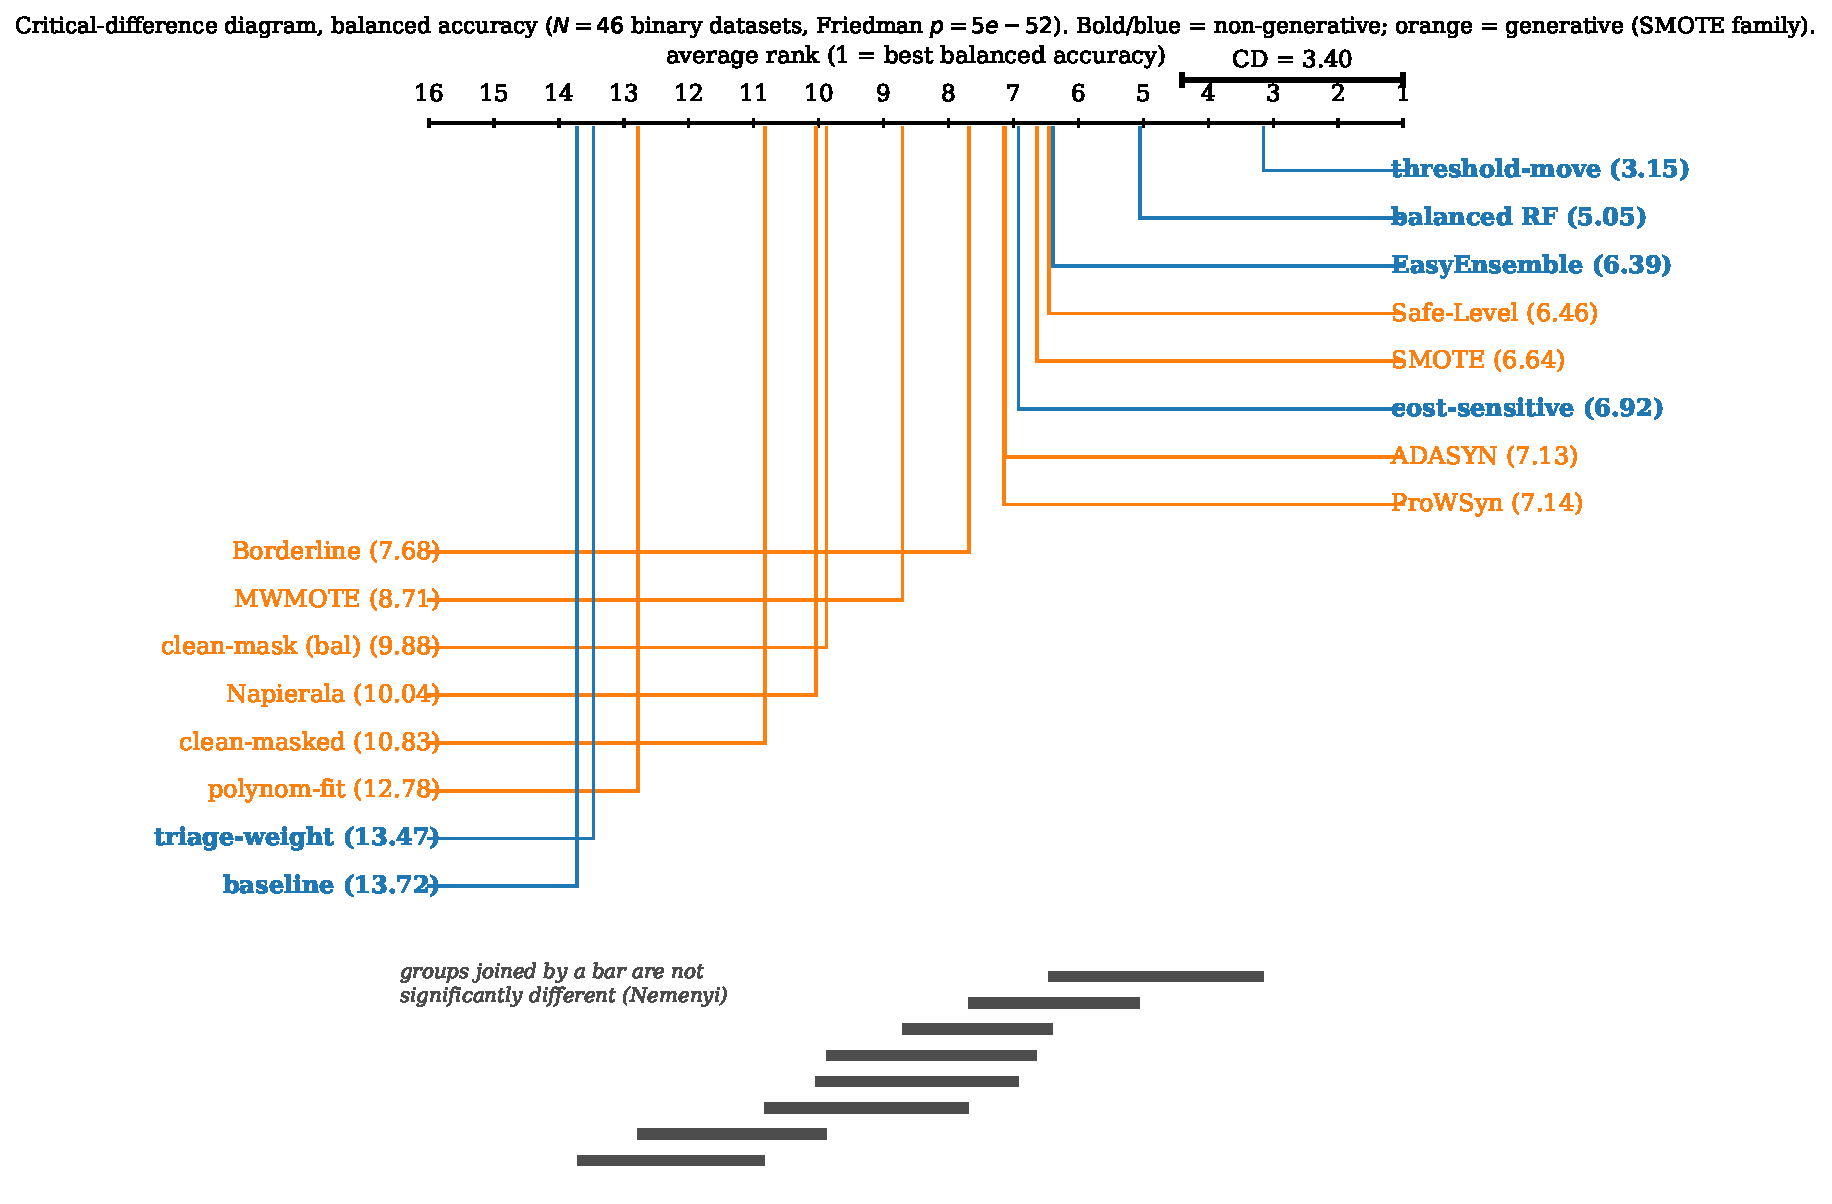
\includegraphics[width=\linewidth]{figures/fig_cd.pdf}
\caption{Critical-difference diagram (Friedman--Nemenyi, $\alpha=0.05$,
$N=46$ binary datasets) of mean per-dataset balanced-accuracy rank over the full
16-strategy menu. Lower rank (right) is better. Non-generative strategies (blue)
threshold-moving, balanced RF, and EasyEnsemble attain the best ranks; the SMOTE
family ranks in the middle; non-rebalancing methods rank worst.}
\label{fig:cd}
\end{figure}

\begin{figure}[t]
\centering
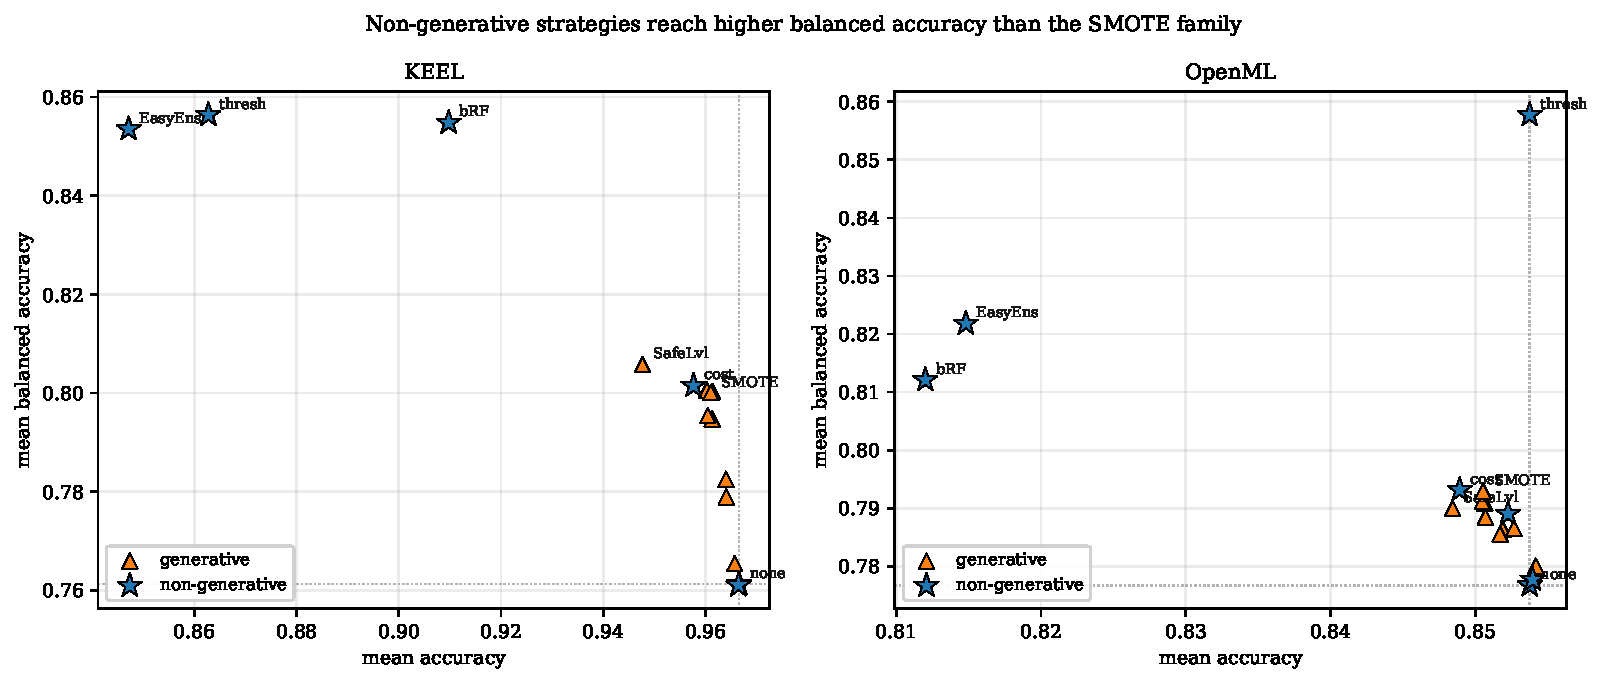
\includegraphics[width=\linewidth]{figures/fig_frontier.pdf}
\caption{Accuracy--balanced-accuracy plane per roster, \emph{at the default
decision threshold}. Non-generative strategies (blue $\star$) reach higher balanced
accuracy than the generative SMOTE family (orange $\triangle$); dotted lines mark
the do-nothing baseline. At threshold parity this gap largely closes
(Table~\ref{tab:parity}).}
\label{fig:frontier}
\end{figure}

\subsection{A regime map: which strategy a dataset needs}\label{sec:results:regime}

\paragraph{Result.} Aggregating the per-dataset oracle choice into five strategy
families, the best move is a balanced ensemble on $42/79$ datasets,
threshold-moving on $17$, cost-sensitive learning on $6$, and \emph{oversampling
on only $12$} ($15\%$); doing nothing is best on $2$. Relative to do-nothing the
mean balanced-accuracy advantage is $+8.1$\,pp for threshold-moving, $+6.1$ for
balanced ensembles, $+3.3$ for oversampling, and $+2.5$ for cost-sensitive
learning. A depth-3 decision tree over the meta-features
(Figure~\ref{fig:regime}) gives an interpretable sketch --- low-separability
(overlapping) data favours balanced ensembles, while large or well-separated data
with a clean minority favours threshold-moving --- but its leave-one-out accuracy
($0.53$) only matches the predict-majority rate, so the map is best read as
\emph{descriptive}: it shows where each family wins, not a rule that beats
``always use a balanced ensemble.''

\begin{figure}[t]
\centering
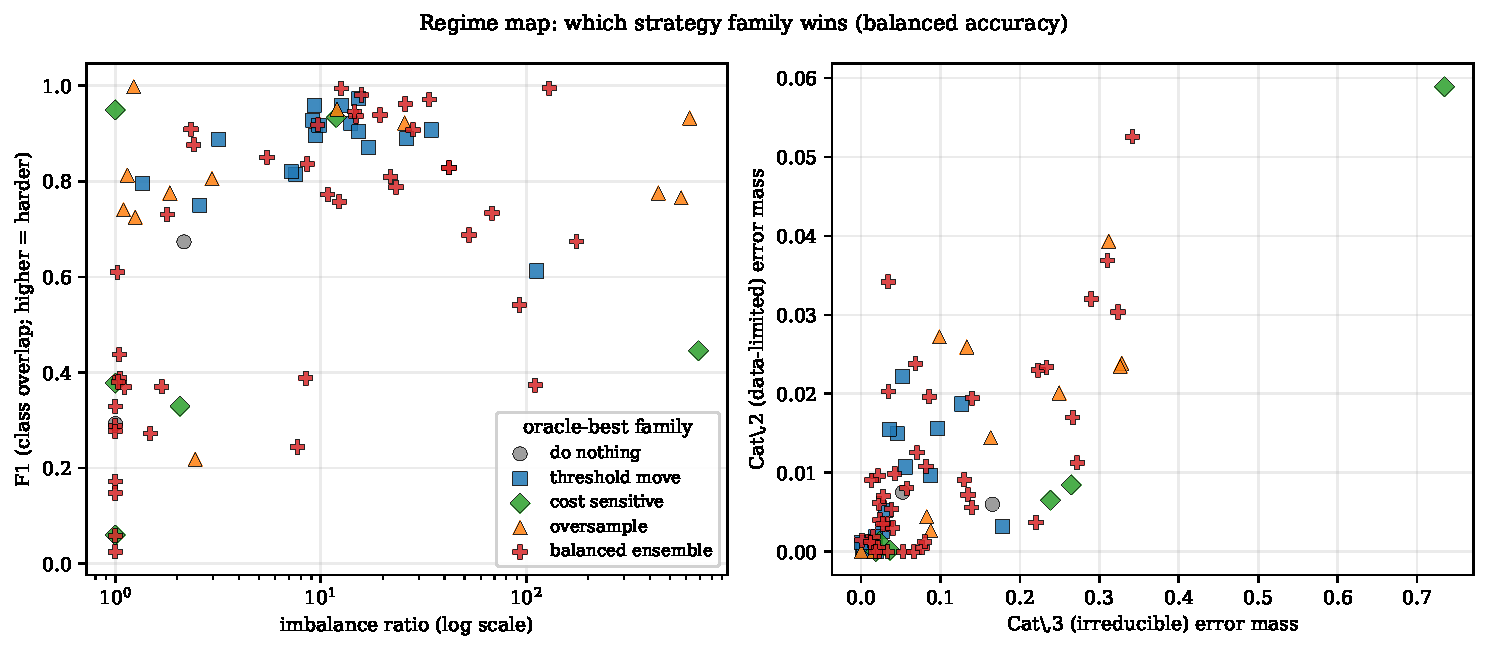
\includegraphics[width=\linewidth]{figures/fig_regime_map.pdf}
\caption{Regime map: the oracle-best strategy family per dataset, over imbalance
ratio vs.\ class overlap (F1, left) and over the triage Cat\,3/Cat\,2 error masses
(right). Oversampling (orange) is best in a minority of regimes; balanced
ensembles and threshold-moving cover most datasets.}
\label{fig:regime}
\end{figure}

\subsection{Prescriptive selection: an honest scope}\label{sec:results:selection}

\paragraph{Result.} Can per-dataset meta-features prescribe the strategy? We train
a leave-one-dataset-out selector on the error-structure and complexity
meta-features and compare it to fixed baselines and an oracle
(Table~\ref{tab:selection}). The selector beats always-SMOTE decisively
($+3.5$\,pp balanced accuracy, $p<10^{-4}$) --- but so does an imbalance-ratio-only
rule, because the gain comes from \emph{having non-generative strategies on the
menu}, not from sophisticated selection. Over the strongest \emph{fixed} strategy
(balanced RF) the edge is real but modest and design-dependent: a direct
method-\emph{classifier} recovers $\sim$60\% of the oracle headroom and robustly
beats best-fixed on balanced accuracy ($+0.64$\,pp, $8/8$ seeds $p\le0.01$) and
G-mean ($+0.64$\,pp, $8/8$ $p\le0.03$), but not MCC; a per-method \emph{regressor}
and the interpretable rule both tie best-fixed.

\begin{table}[t]
\centering
\caption{Prescriptive selection over the full 16-strategy menu, leave-one-dataset-out
across 79 datasets (mean realized metric). A learned selector built on error-structure
and complexity meta-features beats always-SMOTE decisively, but over the strongest
\emph{fixed} strategy its edge is modest: the direct method-classifier robustly beats
best-fixed on balanced accuracy (+0.64\,pp, $8/8$ seeds $p{\le}0.01$) and G-mean
(+0.64\,pp, $8/8$ $p{\le}0.03$) but not MCC; the per-method regressor and an
imbalance-ratio-only rule both tie best-fixed. The dominant lever is the menu, not the
selector.}
\label{tab:selection}
\small
\begin{tabular}{l ccc}
\toprule
Selector / fixed strategy & bal.\ acc & G-mean & MCC \\
\midrule
Oracle (per-dataset best, ceiling)        & 0.838 & 0.866 & 0.696 \\
\midrule
Learned selector --- classifier           & \textbf{0.833} & \textbf{0.862} & 0.677 \\
Learned selector --- regressor            & 0.829 & 0.858 & 0.675 \\
Imbalance-ratio-only selector             & 0.827 & 0.856 & 0.673 \\
\midrule
Best fixed strategy\,$^{a}$               & 0.827 & 0.855 & 0.680 \\
Always-SMOTE                              & 0.795 & 0.827 & 0.678 \\
Baseline (do nothing)                     & 0.772 & 0.805 & 0.670 \\
\bottomrule
\end{tabular}\\[2pt]
{\footnotesize $^{a}$ Best fixed strategy is balanced RF for balanced accuracy and
G-mean, cost-sensitive for MCC.}
\end{table}


\paragraph{Interpretation.} This is a direct, held-out, real-data answer to the
characteristic-driven selection problem left open by \cite{jiang2026beyond}: error-structure
features yield a selector that beats the always-SMOTE paradigm and recovers most
of the achievable gain, but the dominant lever is the \emph{menu}, not selector
sophistication. Indeed, an imbalance-ratio-only selector matches the full
meta-feature selector (Table~\ref{tab:selection}), so the error-structure features
add no measurable \emph{selection} value --- the triage's role here is
explanatory (localizing the boundary for the mechanistic account), not predictive. The
actionable recommendation is therefore simple and robust:
default to a strong non-generative strategy (balanced random forest, or
threshold-moving when calibrated probabilities matter), and reserve oversampling
for the minority of regimes where the map says it wins.

\subsection{Computational cost}\label{sec:results:cost}

The triage (5 forests $\times$ 100 trees) costs $\sim$1\,s on small datasets to
$\sim$33\,s at $n\approx50{,}000$, scaling as $O(n\log n)$ in the training-set size
(dominated by the forest fits; \appref{app:cost}). Crucially it is a \emph{one-time},
classifier-agnostic preprocessing step whose category assignments are reused across
every downstream configuration, fold, and base learner, so over a realistic
model-selection budget it is a small \emph{amortized} cost --- well below the
repeated resample-and-refit it informs, not an added per-model overhead. On very
large datasets the stratified $10{,}000$-instance subsample
(\appref{app:subsampling}) bounds it further without changing the category
distribution, so the triage does not become a bottleneck relative to a single SMOTE
fit.
